\documentclass[
11pt, % The default document font size, options: 10pt, 11pt, 12pt
% codirector, % Uncomment to add a codirector to the title page
]{charter} 

\usepackage{pgfgantt}
\usepackage{xcolor}


% El títulos de la memoria, se usa en la carátula y se puede usar el cualquier lugar del documento con el comando \ttitle
\titulo{Detección de peso de pollos en fincas broiler} 

% Nombre del posgrado, se usa en la carátula y se puede usar el cualquier lugar del documento con el comando \degreename
%\posgrado{Carrera de Especialización en Sistemas Embebidos} 
%\posgrado{Carrera de Especialización en Internet de las Cosas} 
\posgrado{Carrera de Especialización en Inteligencia Artificial}
%\posgrado{Maestría en Sistemas Embebidos} 
%\posgrado{Maestría en Internet de las cosas}
% IMPORTANTE: no omitir titulaciones ni tildación en los nombres, también se recomienda escribir los nombres completos (tal cual los tienen en su documento)
% Tu nombre, se puede usar el cualquier lugar del documento con el comando \authorname
\autor{Ing. Nicolás Martín Tertusio Iglesias}

% El nombre del director y co-director, se puede usar el cualquier lugar del documento con el comando \supname y \cosupname y \pertesupname y \pertecosupname
\director{Ing. Maxim Dorogov}
\pertenenciaDirector{FIUBA} 
\codirector{} % para que aparezca en la portada se debe descomentar la opción codirector en los parámetros de documentclass
\pertenenciaCoDirector{FIUBA}

% Nombre del cliente, quien va a aprobar los resultados del proyecto, se puede usar con el comando \clientename y \empclientename
\cliente{Ing. Marylin Melo de Simons}
\empresaCliente{Empresas Melo S.A.}
 
\fechaINICIO{19 de junio de 2024}		%Fecha de inicio de la cursada de GdP \fechaInicioName
\fechaFINALPlan{17 de agosto de 2024} 	%Fecha de final de cursada de GdP
\fechaFINALTrabajo{31 de enero de 2025}	%Fecha de defensa pública del trabajo final


\begin{document}

\maketitle
\thispagestyle{empty}
\pagebreak

\thispagestyle{empty}
{\setlength{\parskip}{0pt}
\tableofcontents{}
}
\pagebreak


\section*{Registros de cambios}
\label{sec:registro}


\begin{table}[ht]
\label{tab:registro}
\centering
\begin{tabularx}{\linewidth}{@{}|c|X|c|@{}}
\hline
\rowcolor[HTML]{C0C0C0} 
Revisión & \multicolumn{1}{c|}{\cellcolor[HTML]{C0C0C0}Detalles de los cambios realizados} & Fecha      \\ \hline
0      & Creación del documento                                 &\fechaInicioName \\ \hline
1      & Se completa hasta el punto 5 inclusive                 & {26} de {junio} de 2024 \\ \hline
2      & Se completa hasta el punto 9 inclusive                 & {4} de {julio} de 2024 \\ \hline
3      & Se completa hasta el punto 12 inclusive                 & {14} de {julio} de 2024 \\ \hline
4      & Se completa hasta el punto 15 inclusive                 & {23} de {julio} de 2024 \\ \hline
%		  Se puede agregar algo más \newline
%		  En distintas líneas \newline
%		  Así                                                    & {día} de {mes} de 202X \\ \hline
%3      & Se completa hasta el punto 12 inclusive                & {día} de {mes} de 202X \\ \hline
%4      & Se completa el plan	                                 & {día} de {mes} de 202X \\ \hline

% Si hay más correcciones pasada la versión 4 también se deben especificar acá

\end{tabularx}
\end{table}

\pagebreak



\section*{Acta de constitución del proyecto}
\label{sec:acta}

\begin{flushright}
Panamá, \fechaInicioName
\end{flushright}

\vspace{2cm}

Por medio de la presente se acuerda con el \authorname\hspace{1px} que su Trabajo Final de la \degreename\hspace{1px} se titulará ``\ttitle'' y consistirá en la implementación de un sistema de detección de pesos de pollos en finca broiler por medio de \textit{computer vision} (CV). El trabajo tendrá un presupuesto preliminar estimado de 640 horas y un costo estimado de \$19,500.00, con fecha de inicio el \fechaInicioName\hspace{1px} y fecha de presentación pública el \fechaFinalName.

Se adjunta a esta acta la planificación inicial.

\vfill

% Esta parte se construye sola con la información que hayan cargado en el preámbulo del documento y no debe modificarla
\begin{table}[ht]
\centering
\begin{tabular}{ccc}
\begin{tabular}[c]{@{}c@{}}Dr. Ing. Ariel Lutenberg \\ Director posgrado FIUBA\end{tabular} & \hspace{2cm} & \begin{tabular}[c]{@{}c@{}}\clientename \\ \empclientename \end{tabular} \vspace{2.5cm} \\ 
\multicolumn{3}{c}{\begin{tabular}[c]{@{}c@{}} \supname \\ Director del Trabajo Final\end{tabular}} \vspace{2.5cm} \\
\end{tabular}
\end{table}




\section{1. Descripción técnica-conceptual del proyecto a realizar}
\label{sec:descripcion}

% El bloque "consigna" se usa para poner texto en rojo y dar una pequeña ayuda sobre cómo completar la sección. En cada entrega parcial deben eliminar los comandos begin y end del bloque consigna de las secciones que hayan completado.
Empresas Melo S.A. es una empresa de Panamá con una integración vertical en la industria avícola. La compañía se encarga de todo el proceso productivo, desde la creación de alimentos para pollos a partir de materia prima, pasando por la crianza de pollos tipo broiler (de engorde), gallinas ponedoras de huevo y pollos para reproducción, hasta llegar a una planta de sacrificio donde se procesan los pollos según la demanda. Finalmente, los productos pueden ser enviados a una planta de valor agregado donde se crean artículos como milanesas, nuggets, entre otros.

El proyecto se enfoca en el segundo paso: la crianza de los pollos broiler. En las fincas, los pollos se crían en espacios, denominados fincas, que pueden albergar hasta 40.000 aves en 950 m². Actualmente, el peso de los pollos se determina mediante muestreos semanales de 100 a 300 ejemplos, lo que representa menos del 1\% del total, un método que no cumple con los estándares precisos exigidos por el mercado. Para resolver este problema, se propone la instalación de cámaras especializadas en \textit{computer vision} (CV) dentro de las fincas. Estas cámaras capturan imágenes de los pollos y mediante modelos de inteligencia artificial (IA) determinan el peso de cada ave.

En la figura \ref{fig:diagBloques} se presenta el diagrama en bloques del sistema. El proceso comienza con las cámaras de video, que inician la detección de peso mediante el preprocesamiento de las imágenes. Estas imágenes se envían al primer modelo de segmentación y clasificación, cuyo resultado son recortes individuales de cada pollo detectado. A continuación, estos recortes alimentan el segundo modelo de predicción de peso, del cual se obtiene el peso individual de cada ave. Con esta información se calcula el peso promedio de los pollos en la finca y se determina la distribución de los mismos. Los resultados se envían a un sistema de monitoreo y reporte, que junto con la transmisión de video, es accesible para el personal de la finca. Esto permite supervisar el estado de los pollos y determinar el momento adecuado para enviarlos a la planta de sacrificio.

\begin{figure}[htpb]
\centering 
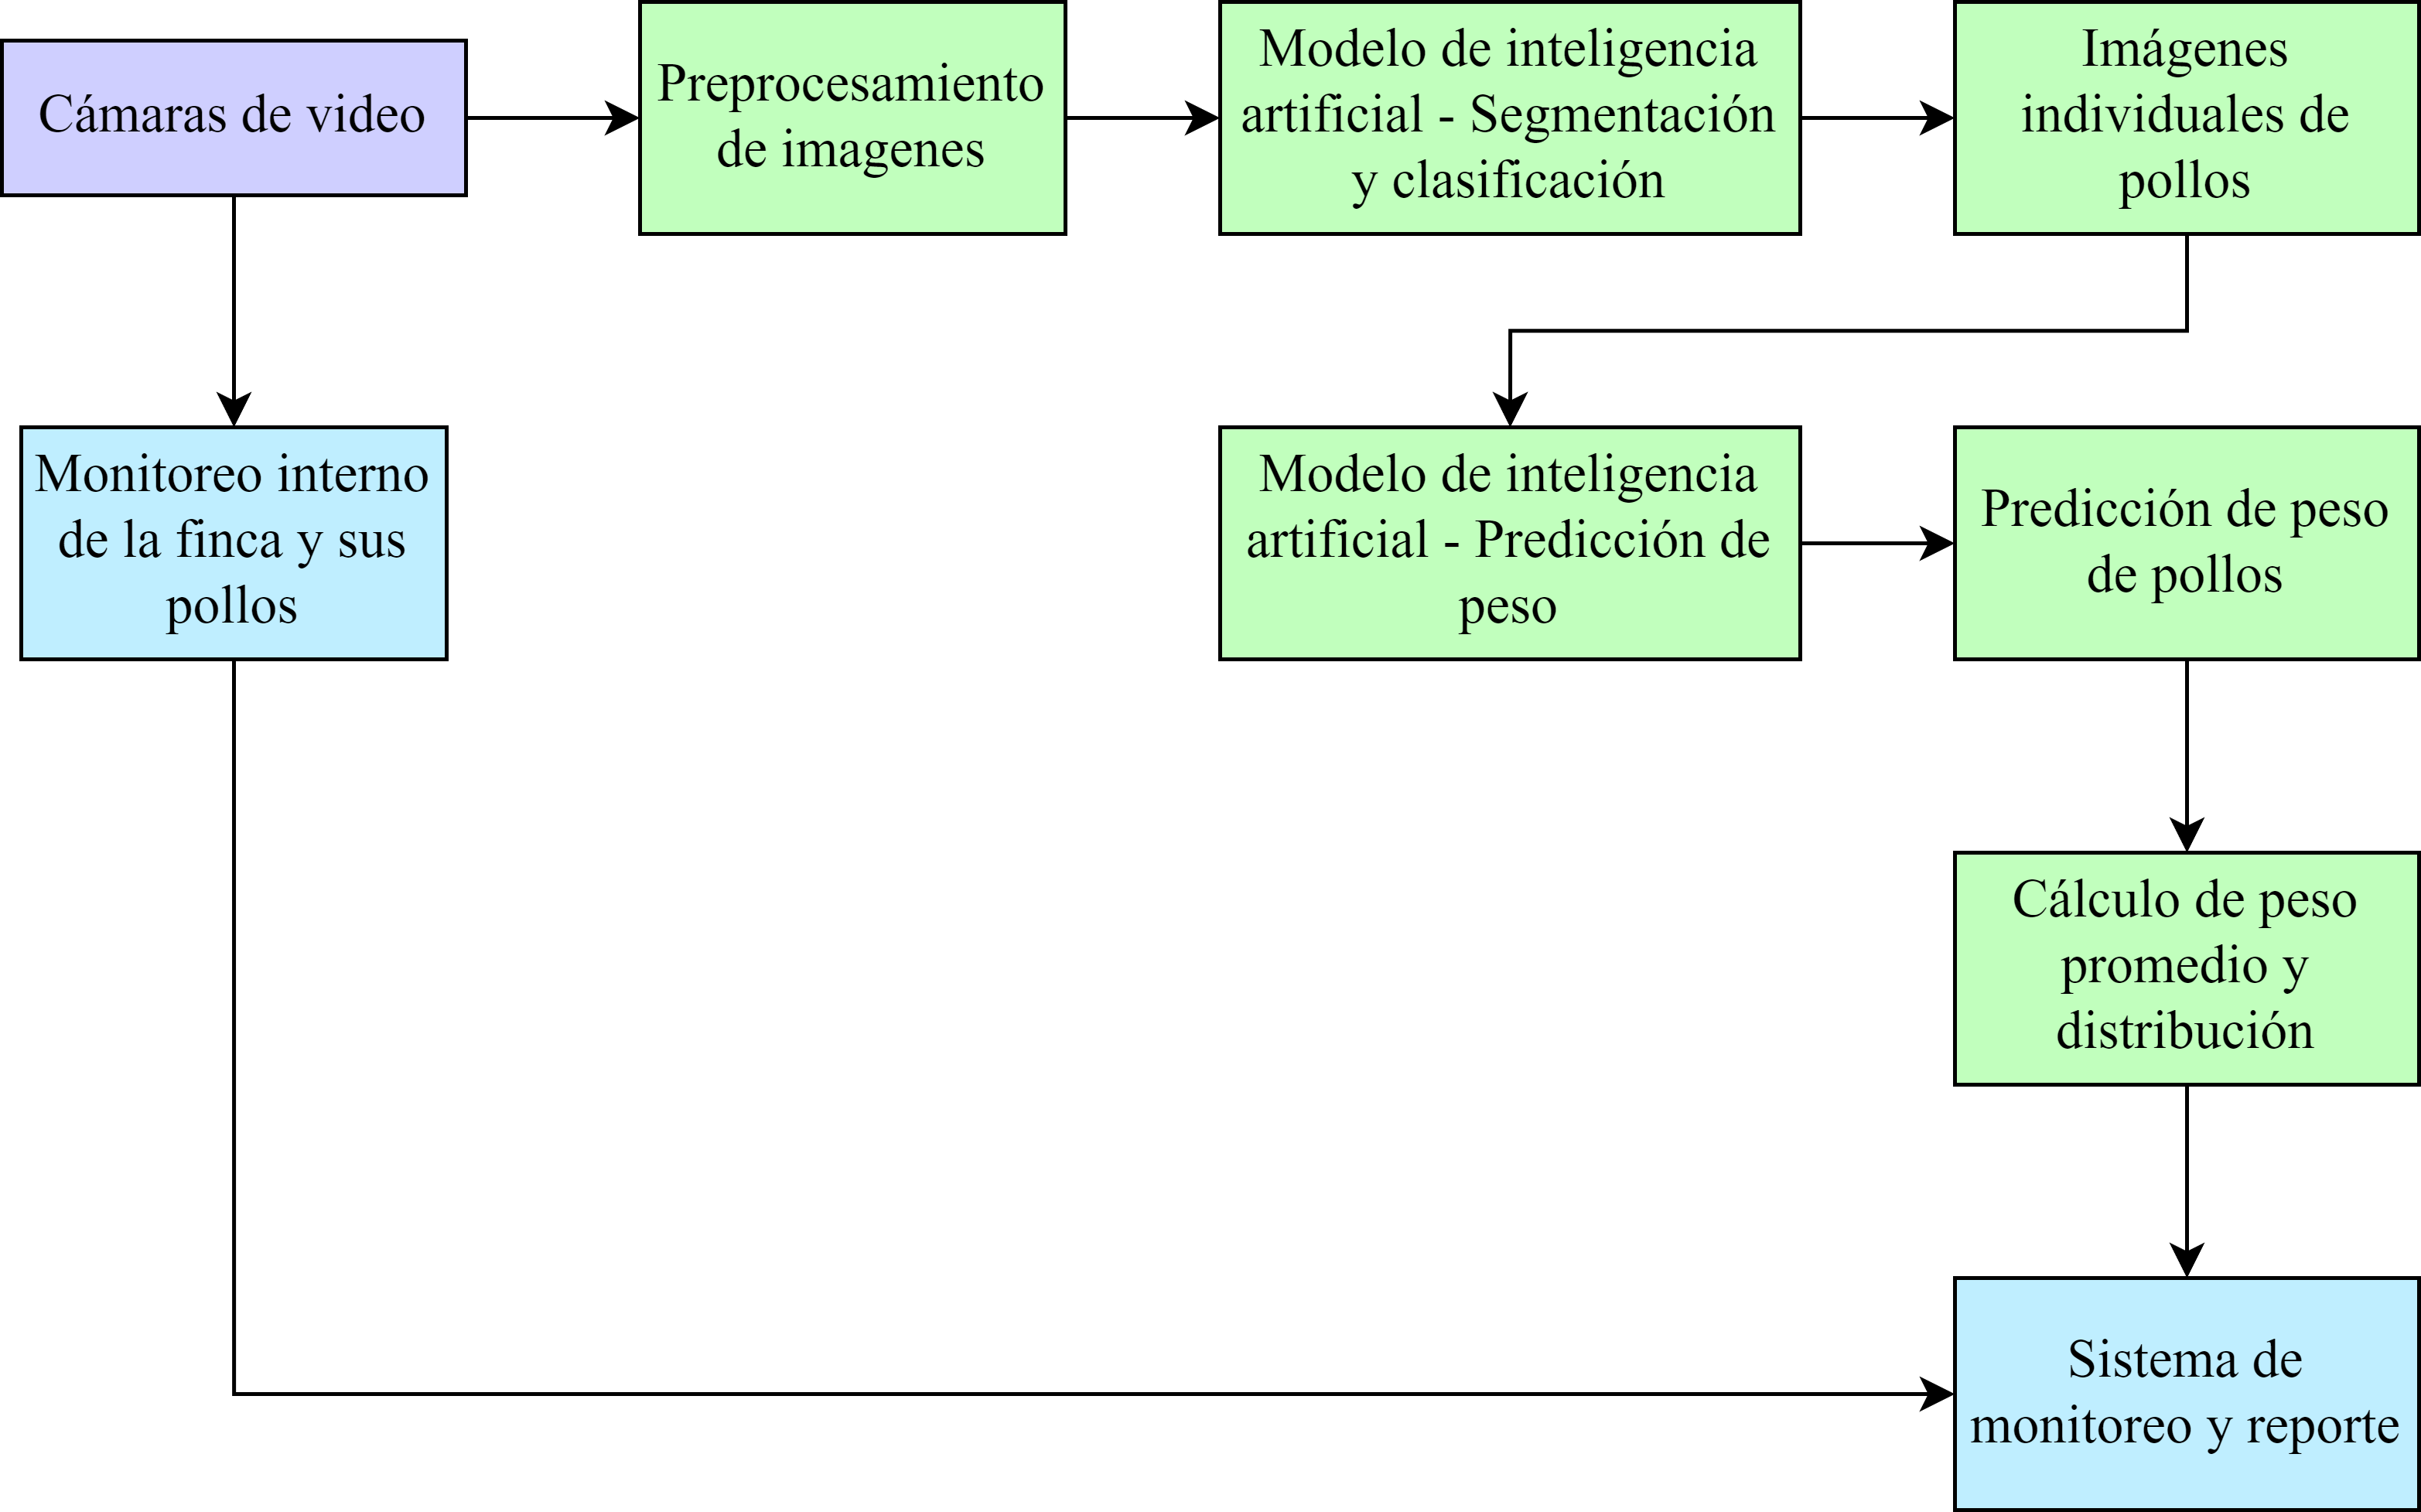
\includegraphics[width=.85\textwidth]{./Figuras/diagBloques2.png}
\caption{Diagrama en bloques del sistema.}
\label{fig:diagBloques}
\end{figure}

\vspace{25px}

\section{2. Identificación y análisis de los interesados}
\label{sec:interesados}

\begin{table}[ht]
%\caption{Identificación de los interesados}
%\label{tab:interesados}
\begin{tabularx}{\linewidth}{@{}|l|X|X|X|@{}}
\hline
\rowcolor[HTML]{C0C0C0} 
Rol           & Nombre y Apellido & Organización 	& Puesto 	\\ \hline
%Auspiciante   &                   &              	&        	\\ \hline
Cliente       & \clientename      &\empclientename	& Directora de operaciones (COO)	\\ \hline
%Impulsor      &                   &              	&        	\\ \hline
Responsable   & \authorname       & FIUBA        	& Alumno 	\\ \hline
Colaboradores & Kelvin Vega       &\empclientename   & Mantenimiento de fincas       	\\ \hline
Orientador    & \supname	      & \pertesupname 	& Director del Trabajo Final \\ \hline
%Equipo        & miembro1 \newline 
%				miembro2          &              	&        	\\ \hline
%Opositores    &                   &              	&        	\\ \hline
Usuario final & Diógenes Becerra         &\empclientename	& Vicepresidente de división Producción       	\\ \hline
\end{tabularx}
\end{table}

\begin{itemize}
	\item Usuario final: se coloca al vicepresidente porque cumple con la figura de representar la división. Sin embargo, los usuarios finales son todo el personal operativo de la finca.
\end{itemize}

\section{3. Propósito del proyecto}
\label{sec:proposito}
El propósito de este proyecto es desarrollar un sistema de monitoreo mediante cámaras de video instaladas en una finca, capaz de predecir el peso de los pollos utilizando técnicas de IA y VC. Este sistema ofrecerá una distribución de peso más precisa que el método de muestreo actual, eliminará el proceso manual de muestreo, permitirá conocer el momento exacto en el que se puede llevar la parvada a la planta de sacrificio y reducirá el consumo de alimento y agua de los pollos.

\section{4. Alcance del proyecto}
\label{sec:alcance}
El proyecto contempla la parte de hardware y software a desarrollar para el diagrama en bloques especificado en la figura \ref{fig:diagBloques}. A desarrollar por el estudiante están las siguientes tareas:

\begin{itemize}
\item Recibir las imágenes de las cámaras de video para iniciar el pipeline de preprocesamiento de las mismas.
\item Implementación de un modelo que, por medio de técnicas de IA y CV, pueda distinguir por lo menos un 80\% de los pollos que se encuentren presentes en una foto.
	\begin{itemize}
	\item Obtención de imágenes para el entrenamiento del modelo seleccionado.
	\item Etiquetado de las imágenes para permitir aprendizaje supervisado.
	\end{itemize}
\item Preprocesamiento de las imágenes de salida del modelo anteriormente mencionado.
\item Implementación de un modelo de IA capaz de predecir, por medio de características físicas y visuales de las aves, el peso de las mismas.
	\begin{itemize}
	\item Al igual que para el primer modelo, se incluye la obtención de imágenes y etiquetado de las mismas.
	\end{itemize}
\item Desarrollo estadístico sobre la distribución de pesos de la parvada.
\item Creación de una interfaz que muestre a los usuarios finales la distribución y peso promedio de los pollos dentro de la finca.
\end{itemize}

A pesar de que está incluido en el alcance del proyecto, no será desarrollado por el estudiante la instalación de cámaras de video. Esto será tercerizado por \empclientename

\section{5. Supuestos del proyecto}
\label{sec:supuestos}
Para el desarrollo del presente proyecto se supone que:

\begin{itemize}
	\item Se dispone de 16 horas semanales para el desarrollo del mismo.
	\item Se tendrá acceso a un stream continuo de video de todas las cámaras instaladas dentro de la finca. 
	\item Se cuenta con una computadora con capacidad computacional suficiente, o un servicio tercerizado similar, para el entrenamiento de los modelos de IA.
	\item Se tendrá disponibilidad limitada para ingresar a la finca y realizar trabajos dentro de la misma, dependiendo de la ocupación de la misma y la naturaleza de los trabajos a realizar.
	\item Se acepta una precisión dentro de un margen razonable de $\pm$10\% para la predicción de pesos de las aves. 
\end{itemize}

\section{6. Requerimientos}
\label{sec:requerimientos}

\begin{enumerate}
	\item Requerimientos de entrenamiento
		\begin{enumerate}
		\item Se debe instalar cámaras de video dentro de la finca.
		\item Se debe recabar la información de entrenamiento de los modelos desde cero y etiquetarla.
		\end{enumerate}
	\item Requerimientos funcionales
		\begin{enumerate}
		\item El sistema debe ser capaz de identificar a un 80\% de pollos que aparecen en cada cámara de video.
		\item El sistema debe ser capaz de segmentar cada una de las aves por medio de coordenadas.
		\item El sistema debe ser capaz de detectar características visuales de cada pollo.
		\item El sistema debe ser capaz de predecir un peso a cada imagen de ave que identifique.
		\end{enumerate}
	\item Requerimientos de documentación
		\begin{enumerate}
		\item Se debe elaborar un informe de avance del proyecto.
		\item Se debe elaborar una memoria técnica del proyecto.
		\item Se debe documentar todo el procesamiento de imágenes que se realice.
		\item El proyecto debe tener un control de versiones por medio de un repositorio de GitHub o alguna herramienta similar.
		\end{enumerate}
	\item Requerimiento de desempeño
		\begin{enumerate}
		\item El procesamiento de video y las detecciones deben ser en tiempo real.
		\item El sistema debe ser capaz de predecir con un margen de $\pm$10\% el peso de cada pollo.
		\end{enumerate}
	\item Requerimientos de la interfaz
		\begin{enumerate}
		\item La interfaz debe mostrar la distribución de pesos de los pollos.
		\item La interfaz debe mostrar el peso promedio estimado de la parvada.
		\item La interfaz debe mostrar el peso promedio de la parvada a lo largo del tiempo.
		\item Se debe poder interactuar con la interfaz para dar inicio a un nuevo lote de pollos.
		\end{enumerate}
\end{enumerate}

\section{7. Historias de usuarios (\textit{Product backlog})}
\label{sec:backlog}

Para el desarrollo del sistema de detección de peso de pollos en fincas broiler, se presentan las siguientes historias de usuario. Cada historia se describe desde la perspectiva del usuario o cliente, indicando claramente el objetivo y la razón detrás de la solicitud.

Además, se ponderan utilizando la escala basada en complejidad, dificultad e incertidumbre, sumando los valores para aproximarlos al siguiente número de la serie de Fibonacci. Por ejemplo, si la complejidad del trabajo es media (5), la dificultad es alta (5) y la incertidumbre es baja (2), los \textit{story points} serían 13 (5 + 5 + 2 = 12, que se aproxima al siguiente número de Fibonacci, que es 13). Los criterios para calcular los \textit{story points} son los siguientes:

\begin{enumerate}
	\item \textbf{Complejidad del trabajo:}
	\begin{itemize}
		\item Alta: 8
		\item Media: 5
		\item Baja: 2
	\end{itemize}
	\item \textbf{Dificultad del trabajo:}
	\begin{itemize}
		\item Alta: 5
		\item Media: 3
		\item Baja: 2
	\end{itemize}
	\item \textbf{Incertidumbre del trabajo:}
	\begin{itemize}
		\item Alta: 8
		\item Media: 3
		\item Baja: 2
	\end{itemize}
\end{enumerate}

\textbf{Historias de usuario:}

\begin{enumerate}
\item Como gerente de producción, quiero ver la evolución del peso promedio de la parvada a lo largo del tiempo en la interfaz, para detectar tendencias y hacer ajustes en la crianza.

\textit{Story points}: 8 (complejidad: 2, dificultad: 2, incertidumbre: 2)

\item Como supervisor de la finca, quiero interactuar con la interfaz del sistema para iniciar un nuevo lote de pollos, para asegurar un manejo ordenado y documentado de cada ciclo de producción.

\textit{Story points}: 8 (complejidad: 2, dificultad: 2, incertidumbre: 3)

\item Como trabajador de la finca, quiero que el sistema prediga el peso de cada pollo basado en las imágenes, para tomar decisiones informadas sobre el momento adecuado para llevar las aves a la planta de sacrificio.

\textit{Story points}: 21 (complejidad: 8, dificultad: 5, incertidumbre: 3)

\item Como gerente de operaciones, quiero que se guarde la información al iniciar un lote nuevo, para llevar un histórico de parvadas anteriores.

\textit{Story points}: 21 (complejidad: 5, dificultad: 3, incertidumbre: 8)

\end{enumerate}

\section{8. Entregables principales del proyecto}
\label{sec:entregables}

Los entregables del proyecto son (ejemplo):

\begin{itemize}
	\item Informe de avance del proyecto.
	\item Manual de usuario.
	\item Código fuente del firmware.
	\item Interfaz web para ver el peso promedio, cambio en el tiempo de la misma y distribución de pesos actual.
	\item Memoria del trabajo final.
\end{itemize}

\section{9. Desglose del trabajo en tareas}
\label{sec:wbs}

\begin{enumerate}
\item Compra de equipos (35 horas)
	\begin{enumerate}
	\item Comprar las cámaras de video a utilizar e instalarlas dentro de la finca. (32 horas)
	\item Comprar un ordenador o contratar un servicio en la nube para el entrenamiento de los modelos de IA. (asíncrono, 3 horas)
	\end{enumerate}
\item Toma de datos (170 horas)
	\begin{enumerate}
	\item Capturar imágenes de pollos en diferentes condiciones de iluminación y ángulos. (70 horas)
	\item Capturar imágenes de pollos junto con mediciones precisas de su peso. (70 horas)
	\item Control de calidad de imágenes capturadas: clasificación, ordenamiento, asegurar cantidades suficientes y variadas de imágenes para un entrenamiento correcto de los modelos de IA. (30 horas)
	\end{enumerate}
\item Etiquetado de datos (30 horas)
	\begin{enumerate}
	\item Utilizar software de etiquetado para marcar y clasificar cada pollo en las imágenes. (15 horas)
	\item Asociar cada imagen con el peso real del pollo. (15 horas)
	\end{enumerate}
\item Desarrollo del pipeline de preprocesamiento (30 horas)
	\begin{enumerate}
	\item Escribir códigos para limpiar y preparar las imágenes. (20 horas)
	\item Aplicar técnicas de aumento de datos para mejorar la robustez del modelo. (10 horas)
	\end{enumerate}
\item Entrenamiento del modelo de segmentación y clasificación (120 horas)
	\begin{enumerate}
	\item Seleccionar y configurar el modelo de IA apropiado. (20 horas)
	\item Entrenar el modelo utilizando las imágenes etiquetadas. (100 horas)
	\end{enumerate}
\item Entrenamiento del modelo de predicción de peso (75 horas)
	\begin{enumerate}
	\item Seleccionar y configurar el modelo de IA apropiado. (15 horas)
	\item Entrenar el modelo utilizando las imágenes etiquetadas con peso. (60 horas)
	\end{enumerate}
\item Desarrollo de la interfaz web (75 horas)
	\begin{enumerate}
	\item Desarrollar la interfaz utilizando tecnologías web. (15 horas)
	\item Integrar el backend para mostrar datos en tiempo real. (25 horas)
	\item Implementar gráficos para mostrar el peso promedio. (5 horas)
	\item Implementar gráficos históricos para mostrar la evolución del peso. (5 horas)
	\item Desarrollar funcionalidad para iniciar y gestionar nuevos lotes de pollos. (5 horas)
	\item Realizar pruebas de usabilidad con los usuarios finales. (20 horas)
	\end{enumerate}
\item Documentación (65 horas)
	\begin{enumerate}
	\item Documentar el informe de avance del proyecto. (20 horas)
	\item Documentar la memoria técnica del proyecto. (20 horas)
	\item Documentar el etiquetado y preprocesamiento de imágenes. (15 horas)
	\item Documentar el entrenamiento y evaluación de los modelos de IA. (35 horas)
	\item Documentar el desarrollo e implementación de la interfaz web. (15 horas)
	\end{enumerate}
\end{enumerate}

Cantidad total de horas: 640 horas.

\section{10. Diagrama de Activity On Node}
\label{sec:AoN}

En la figura \ref{fig:AoN} se muestra el diagrama \textit{Activity on Node} con las dependencias de las tareas del proyecto. Los grupos de actividades se identifican con diferentes colores como está descrito en la figura \ref{fig:LegendAoN}.

\begin{figure}[htpb]
\centering 
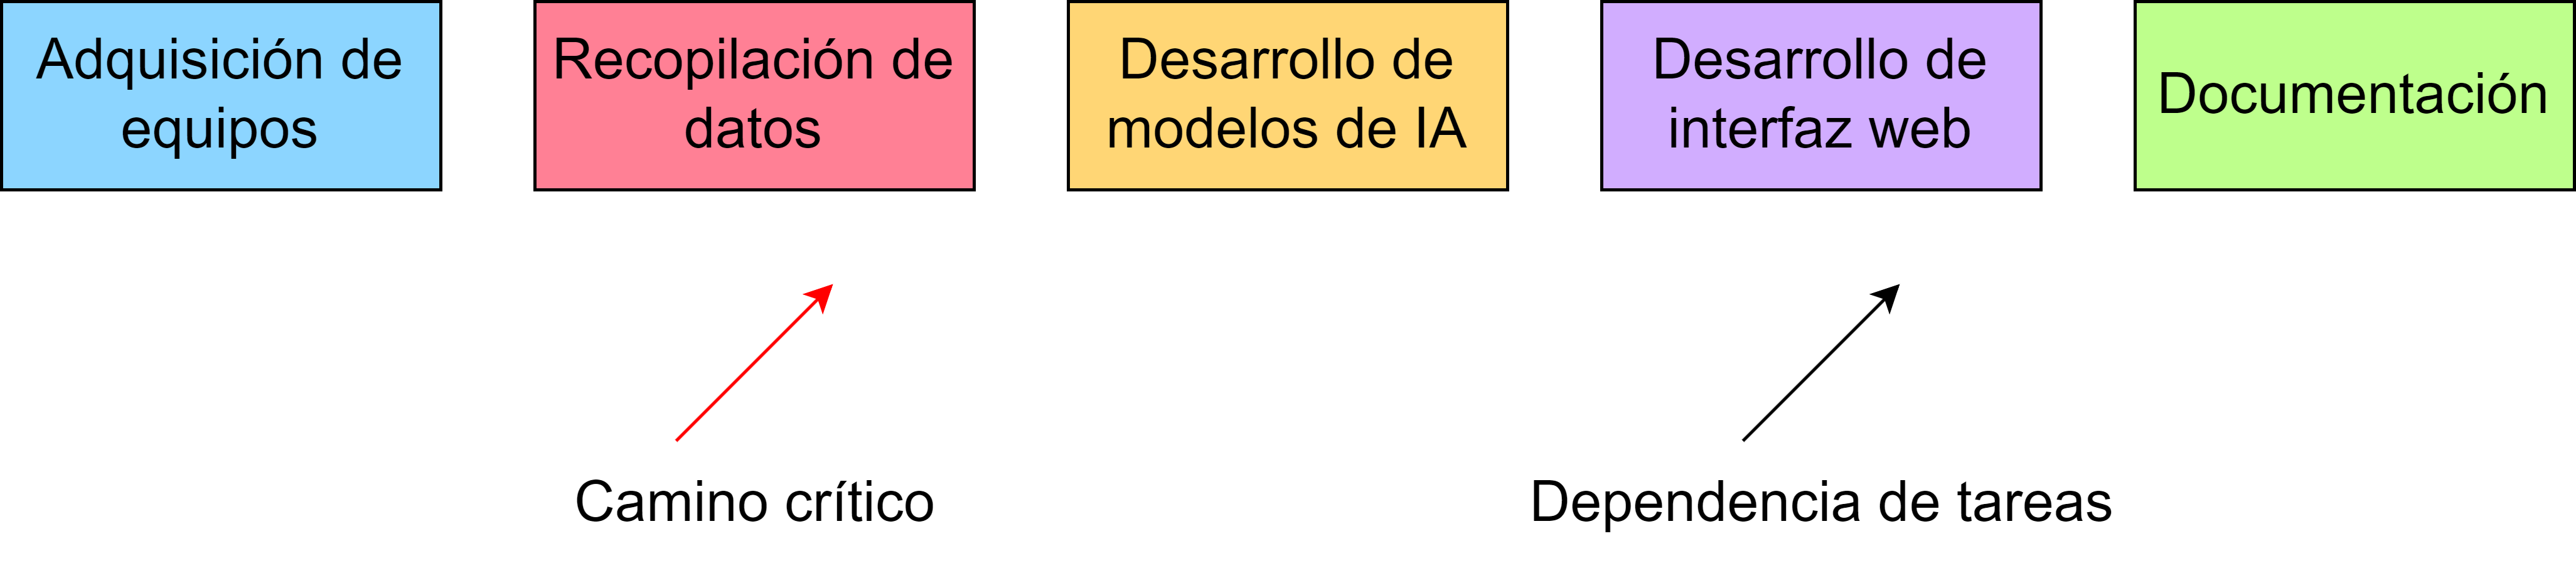
\includegraphics[width=.8\textwidth]{./Figuras/Legend Activity on Node.png}
\caption{Cuadro indicativo del diagrama de \textit{Activity on Node}.}
\label{fig:LegendAoN}
\end{figure}

\begin{figure}[htpb]
\centering 
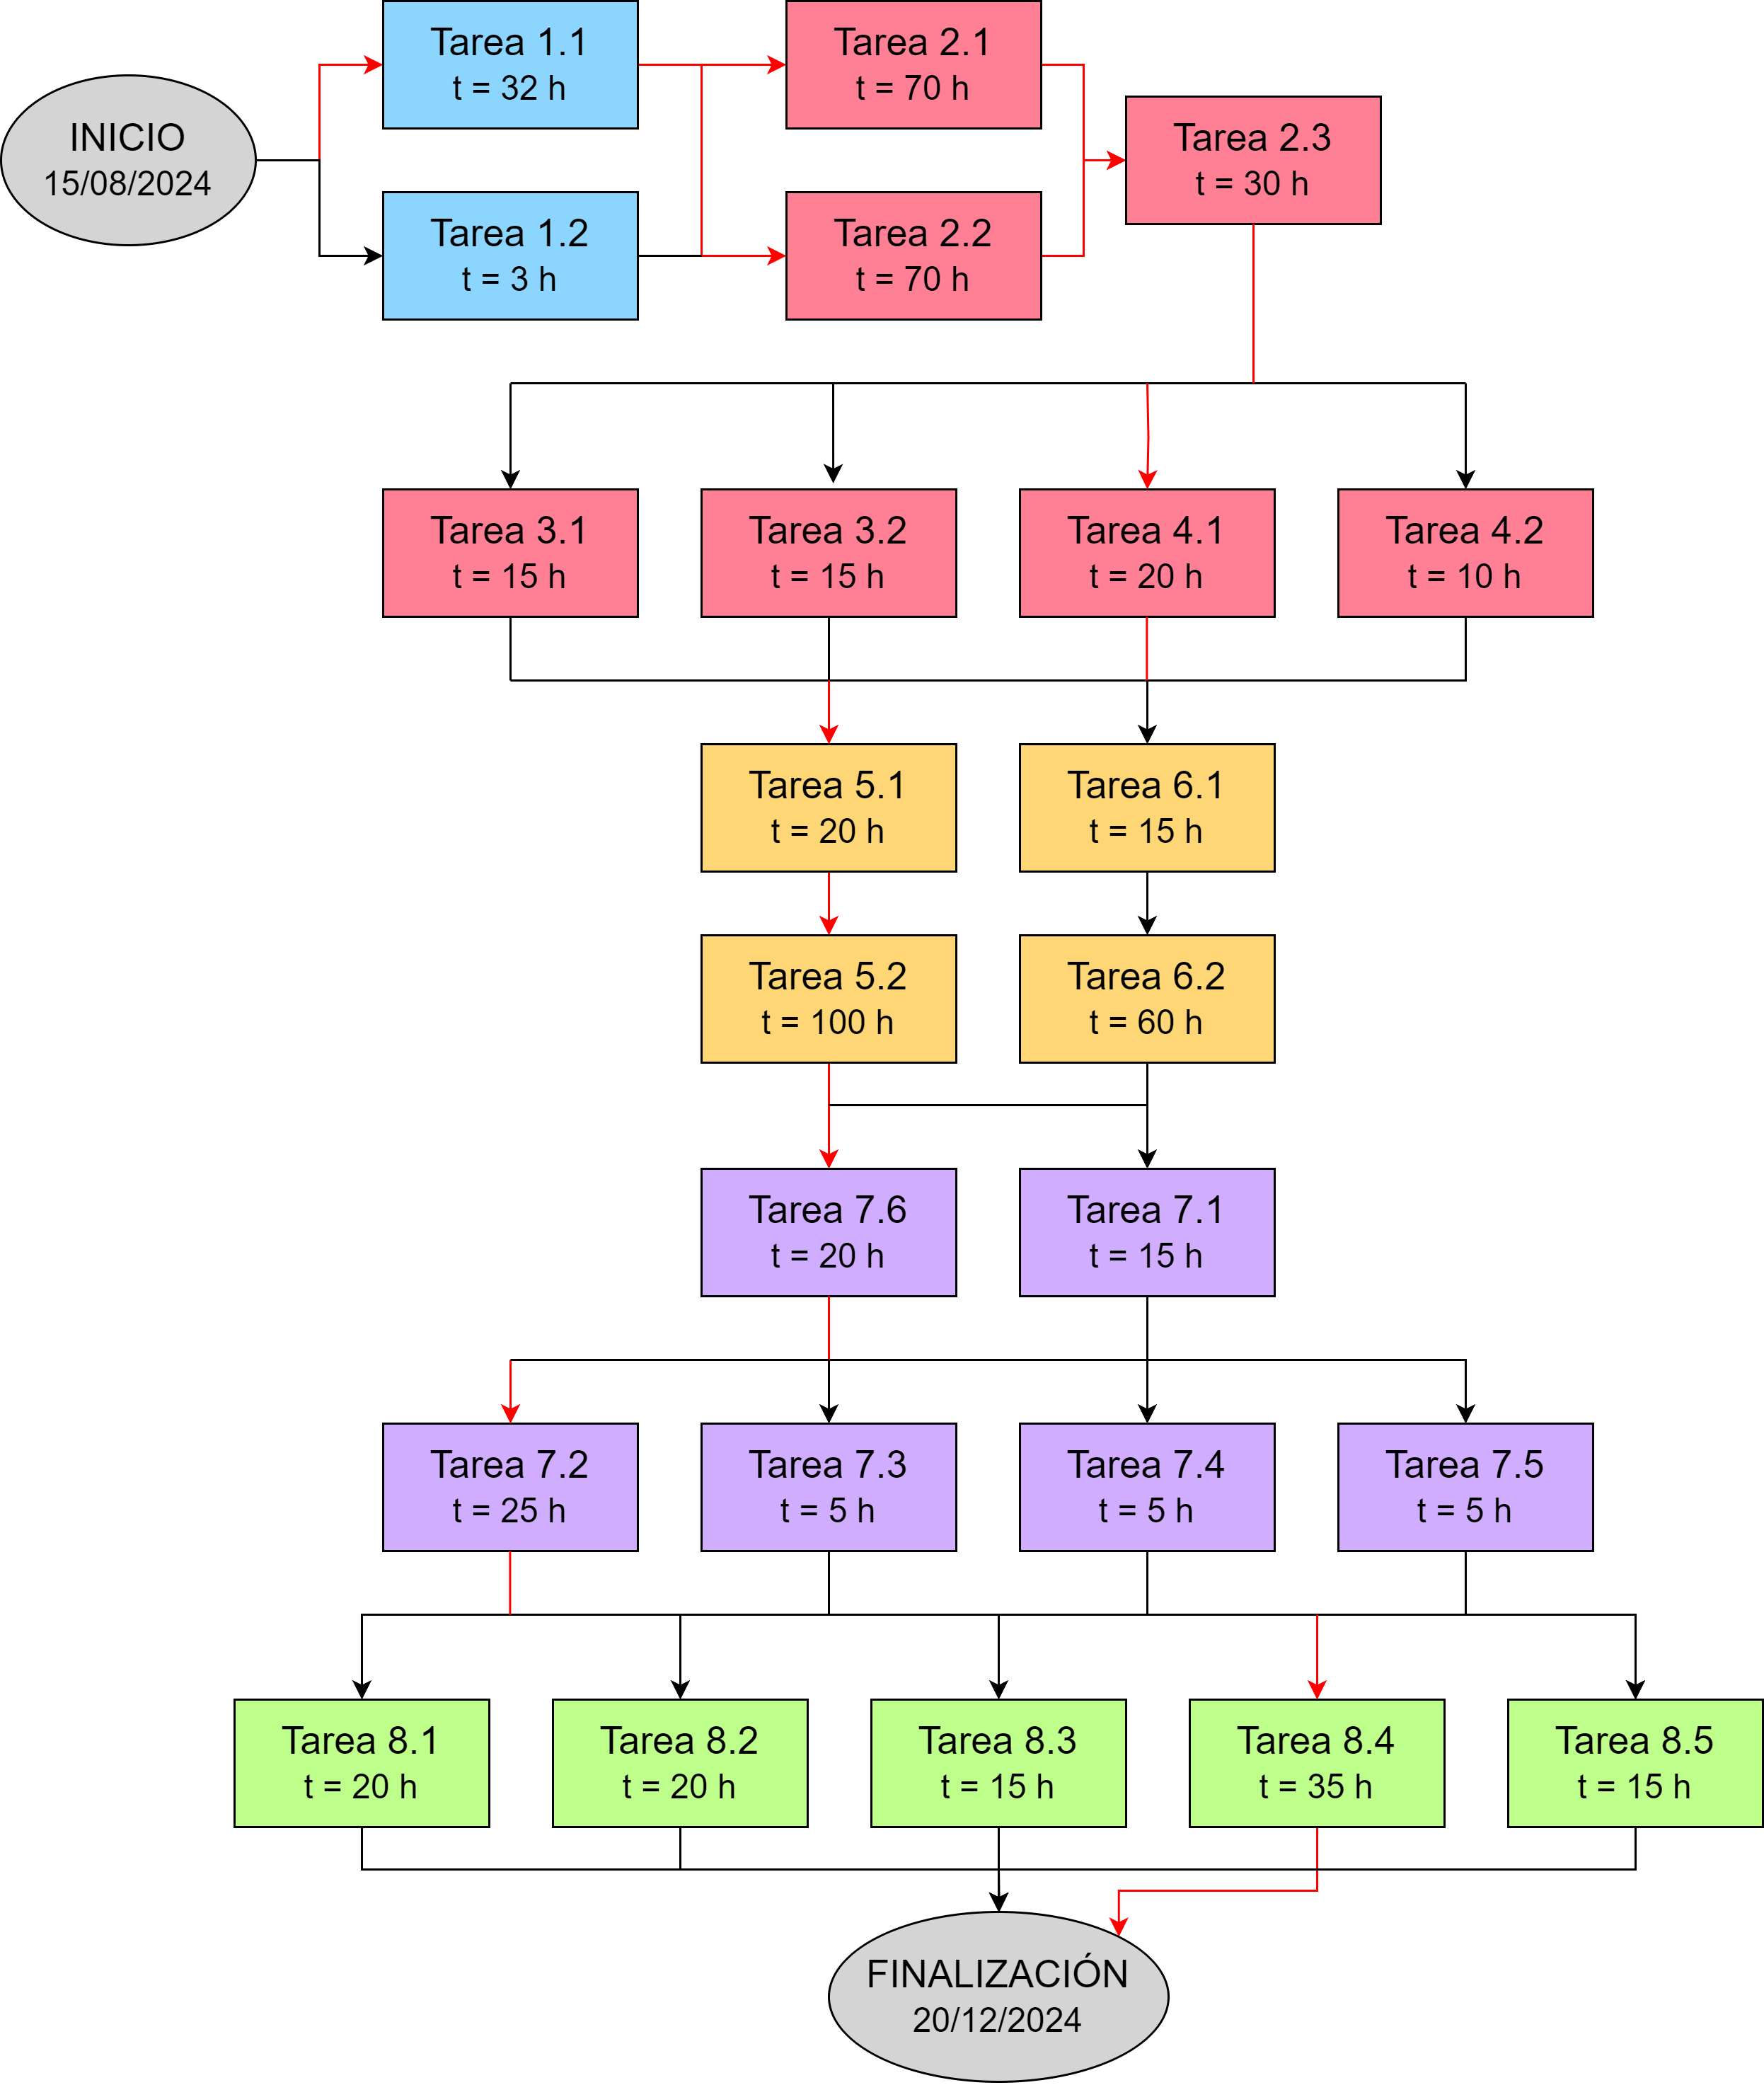
\includegraphics[width=.8\textwidth]{./Figuras/Activity on Node.png}
\caption{Diagrama de \textit{Activity on Node}.}
\label{fig:AoN}
\end{figure}

\section{11. Diagrama de Gantt}
\label{sec:gantt}

En la figura \ref{fig:gantt} se muestra el diagrama de Gantt del proyecto.

\begin{landscape}
\begin{figure}[htpb]
\begin{center}
\ganttset{%
        calendar week text={%
            S\currentweek
        }%
    }
\begin{ganttchart}[
    vgrid,
    hgrid,
    x unit=0.125cm,
    y unit title=0.6cm,
    y unit chart=0.45cm,
    milestone/.append style={xscale=4},
    title height=1,
    time slot unit=day,
    time slot format=isodate,
    title/.append style={fill=blue!50},
    title label font=\color{white}\bfseries,
    canvas/.append style={fill=white},
    bar/.append style={draw=black,fill=blue!30},
    bar incomplete/.append style={fill=red!30},
    bar label font=\color{black},
    group/.append style={fill=black!70, draw=black},
]{2024-08-15}{2025-01-31}
    \gantttitlecalendar{year, month, week=1} \\

    
    % Compra de equipos
    \ganttgroup{Equipos}{2024-08-15}{2024-08-25} \\
    \ganttbar{Tarea 1.1}{2024-08-15}{2024-08-25} \\
    \ganttbar{Tarea 1.2}{2024-08-15}{2024-08-25} \\

    % Toma de datos
    \ganttgroup{Toma de datos}{2024-08-26}{2024-10-14} \\
    \ganttbar{Tarea 2.1}{2024-08-26}{2024-10-07} \\
    \ganttbar{Tarea 2.2}{2024-08-26}{2024-10-07} \\
    \ganttbar{Tarea 2.3}{2024-09-01}{2024-10-14} \\

    % Etiquetado de datos
    \ganttgroup{Etiquetado}{2024-10-14}{2024-10-31} \\
    \ganttbar{Tarea 3.1}{2024-10-14}{2024-10-31} \\
    \ganttbar{Tarea 3.2}{2024-10-17}{2024-10-31} \\

    % Desarrollo del pipeline de preprocesamiento
    \ganttgroup{Procesamiento}{2024-10-14}{2024-11-03} \\
    \ganttbar{Tarea 4.1}{2024-10-14}{2024-11-03} \\
    \ganttbar{Tarea 4.2}{2024-10-14}{2024-11-03} \\

    % Entrenamiento del modelo de segmentación y clasificación
    \ganttgroup{Entrenamiento}{2024-11-04}{2024-11-30} \\
    \ganttbar{Tarea 5.1}{2024-11-04}{2024-11-25} \\
    \ganttbar{Tarea 5.2}{2024-11-11}{2024-11-30} \\
    \ganttbar{Tarea 6.1}{2024-11-10}{2024-11-25} \\
    \ganttbar{Tarea 6.2}{2024-11-15}{2024-11-30} \\

    % Desarrollo de la interfaz web
    \ganttgroup{Interfaz web}{2024-12-01}{2024-12-15} \\
    \ganttbar{Tarea 7.1}{2024-12-01}{2024-12-05} \\
    \ganttbar{Tarea 7.2}{2024-12-01}{2024-12-15} \\
    \ganttbar{Tarea 7.3}{2024-12-01}{2024-12-08} \\
    \ganttbar{Tarea 7.4}{2024-12-01}{2024-12-10} \\
    \ganttbar{Tarea 7.5}{2024-12-01}{2024-12-12} \\
    \ganttbar{Tarea 7.6}{2024-12-01}{2024-12-15} \\

    % Documentación
    \ganttgroup{Documentos}{2024-12-15}{2025-01-31} \\
    \ganttbar{Tarea 8.1}{2024-12-15}{2025-01-31} \\
    \ganttbar{Tarea 8.2}{2024-12-15}{2025-01-31} \\
    \ganttbar{Tarea 8.3}{2024-12-15}{2025-01-31} \\
    \ganttbar{Tarea 8.4}{2024-12-15}{2025-01-31} \\
    \ganttbar{Tarea 8.5}{2024-12-15}{2025-01-31} \\

\end{ganttchart}
\end{center}
\caption{Diagrama de Gantt.}
\label{fig:gantt}
\end{figure}
\end{landscape}


\section{12. Presupuesto detallado del proyecto}
\label{sec:presupuesto}

A continuación, se presenta el análisis de costos del proyecto expresado en dólares estadounidenses (USD). La tasa de conversión al día 15 de julio de 2024 establece que \$922.24 ARS equivale a \$1.00 USD.

\begin{table}[htpb]
\centering
\begin{tabularx}{\linewidth}{@{}|X|c|r|r|@{}}
\hline
\rowcolor[HTML]{C0C0C0} 
\multicolumn{4}{|c|}{\cellcolor[HTML]{C0C0C0}COSTOS DIRECTOS} \\ \hline
\rowcolor[HTML]{C0C0C0} 
Descripción &
  \multicolumn{1}{c|}{\cellcolor[HTML]{C0C0C0}Cantidad} &
  \multicolumn{1}{c|}{\cellcolor[HTML]{C0C0C0}Valor unitario} &
  \multicolumn{1}{c|}{\cellcolor[HTML]{C0C0C0}Valor total} \\ \hline
 
  \multicolumn{1}{|l|}{Cámaras para CV} & 
  \multicolumn{1}{c|}{5} &
  \multicolumn{1}{c|}{\$300.00} &
  \multicolumn{1}{c|}{\$1,500.00} \\ \hline
  
  \multicolumn{1}{|l|}{Instalación de cámaras y materiales} & 
  \multicolumn{1}{c|}{1} &
  \multicolumn{1}{c|}{\$4,000.00} &
  \multicolumn{1}{c|}{\$4,000.00} \\ \hline
  
  \multicolumn{1}{|l|}{Computadora para entrenamiento de modelos} & 
  \multicolumn{1}{c|}{1} &
  \multicolumn{1}{c|}{\$4,000.00} &
  \multicolumn{1}{c|}{\$4,000.00} \\ \hline
  
  \multicolumn{3}{|c|}{SUBTOTAL} &
  \multicolumn{1}{c|}{\$9,500.00} \\ \hline
  \rowcolor[HTML]{C0C0C0} 
  \multicolumn{4}{|c|}{\cellcolor[HTML]{C0C0C0}COSTOS INDIRECTOS} \\ \hline
  \rowcolor[HTML]{C0C0C0} 
Descripción &
  \multicolumn{1}{c|}{\cellcolor[HTML]{C0C0C0}Cantidad} &
  \multicolumn{1}{c|}{\cellcolor[HTML]{C0C0C0}Valor unitario} &
  \multicolumn{1}{c|}{\cellcolor[HTML]{C0C0C0}Valor total} \\ \hline
 
  \multicolumn{1}{|l|}{Meses de consumo eléctrico de equipos} & 
  \multicolumn{1}{c|}{4} &
  \multicolumn{1}{c|}{\$100.00} &
  \multicolumn{1}{c|}{\$400.00} \\ \hline
  
  \multicolumn{1}{|l|}{Horas de trabajo} & 
  \multicolumn{1}{c|}{640} &
  \multicolumn{1}{c|}{\$15.00} &
  \multicolumn{1}{c|}{\$9,600.00} \\ \hline

\multicolumn{3}{|c|}{SUBTOTAL} &
  \multicolumn{1}{c|}{\$10,000.00} \\ \hline
\rowcolor[HTML]{C0C0C0}
\multicolumn{3}{|c|}{TOTAL} &
\multicolumn{1}{c|}{\$19,500.00} \\ \hline
\end{tabularx}%
\end{table}


\section{13. Gestión de riesgos}
\label{sec:riesgos}

A continuación se listan los potenciales riesgos que se podrían presentar en el desarrollo del proyecto. Para la estimación de la severidad (S) y la probabilidad de ocurrencia (O) de los riesgos se utiliza una escala del 1 al 10, donde 1 es el valor mínimo y 10 es el valor máximo.

a) Identificación de los riesgos (al menos cinco) y estimación de sus consecuencias:
 
Riesgo 1: Poder computacional reducido para entrenamiento de modelos.
\begin{itemize}
	\item Severidad (S): 5. \\
	Riesgo de severidad media, la repercusión de no contar con gran poder computacional afecta los tiempos de entrenamiento mas no el desempeño de los modelos.
	\item Probabilidad de ocurrencia (O): 2. \\
	Se hará una investigación previa sobre los requisitos computacionales y el equipo a comprar/servicio a contratar, por lo que la posibilidad de este riesgo es baja.
\end{itemize}   

Riesgo 2: Retrasos en la entrega e instalación de equipos.
\begin{itemize}
	\item Severidad (S): 3. \\
	Riesgo de severidad baja, ya que se pueden ir adelantando otras tareas mientras los equipos se compran y son instalados.
	\item Probabilidad de ocurrencia (O): 7. \\
	Los proveedores pueden experimentar problemas logísticos, especialmente en contextos internacionales, por lo que se asigna una probabilidad alta.
\end{itemize}

Riesgo 3: Problemas de conectividad.
\begin{itemize}
	\item Severidad (S):  7.\\
	La pérdida de conectividad puede interrumpir la transmisión de datos en tiempo real, afectando la capacidad de respuesta del sistema.
	\item Probabilidad de ocurrencia (O): 5.\\
	Las fincas pueden tener problemas de conectividad debido a infraestructura limitada por su naturaleza rural.
\end{itemize}

Riesgo 4: Deterioro de cámaras dentro de la finca.
\begin{itemize}
	\item Severidad (S):  8.\\
	Las cámaras son fundamentales para el desarrollo el proyecto ya que ellas son las que obtienen los datos de entrada de los modelos de IA.
	\item Probabilidad de ocurrencia (O): 6.\\
	El ambiente dentro de la finca es hostil para componentes electrónicos por la gran humedad en aire y orina de los pollos.
\end{itemize}

Riesgo 5: Precisión baja del sistema para detectar peso de los pollos.
\begin{itemize}
	\item Severidad (S):  8.\\
	El objetivo principal del sistema es determinar el momento perfecto para llevar los pollos a la planta de sacrificio, una baja precisión llevaría a perdidas o insatisfacción de los clientes.
	\item Probabilidad de ocurrencia (O): 3.\\
	La precisión de los modelos se compara con los métodos actuales de muestreo, los cuales no son representativos de la parvada. El estado del arte en cuanto a modelos de IA para segmentación de instancias y detección de features son prometedores.
\end{itemize}


b) Tabla de gestión de riesgos:      (El RPN se calcula como RPN=SxO)

\begin{table}[htpb]
\centering
\begin{tabularx}{\linewidth}{@{}|X|c|c|c|c|c|c|@{}}
\hline
\rowcolor[HTML]{C0C0C0} 
Riesgo & S & O & RPN & S* & O* & RPN* \\ \hline
Poder computacional reducido para entrenamiento de modelos.       & 5  &  2 & 10    & -   &  -  & -     \\ \hline
Retrasos en la entrega e instalación de equipos.       & 3  & 7  & 21    & -   & -   & -     \\ \hline
Problemas de conectividad.       & 7  & 5  &  35   & 3   & 5   &  15    \\ \hline
Deterioro de cámaras dentro de la finca.       & 8  & 6  &  48   & 8   & 1   & 8     \\ \hline
Precisión baja del sistema para detectar peso de los pollos.       & 8  & 3  &   24  & -   &  -  &   -   \\ \hline
\end{tabularx}%
\end{table}

Criterio adoptado: 

Se tomarán medidas de mitigación en los riesgos cuyos números de RPN sean mayores a 25.

Nota: los valores marcados con (*) en la tabla corresponden luego de haber aplicado la mitigación.

c) Plan de mitigación de los riesgos que originalmente excedían el RPN máximo establecido:
 
Riesgo 3: Desarrollar la interfaz del sistema de modo que se pueda acceder a ella tanto remota como localmente.
  \begin{itemize}
	\item Severidad (S*): 3.
          El personal de la finca utiliza medios que no requieren Internet para comunicarse entre ellos, por lo que se puede revisar el sistema localmente en la finca en caso de perdidas de conexión.
	\item Probabilidad de ocurrencia (O*): 5.
          La ocurrencia de los problemas de conexión son por la naturaleza rural de las fincas y disminuirlo implicaría hablar con los proveedores del servicio, lo cual escapa del alcance del proyecto.
	\end{itemize}

Riesgo 4: Comprar cámaras diseñadas para entornos hostiles.
  \begin{itemize}
	\item Severidad (S*): 8.
          Daños en las cámaras sigue siendo devastador para el sistema.
	\item Probabilidad de ocurrencia (O*): 1.
          Cámaras con protección adecuada, por ejemplo IP67, reducen significativamente la posibilidad de daños en las mismas.
	\end{itemize}



\section{14. Gestión de la calidad}
\label{sec:calidad}

Elija al menos diez requerimientos que a su criterio sean los más importantes/críticos/que aportan más valor y para cada uno de ellos indique las acciones de verificación y validación que permitan asegurar su cumplimiento.

\begin{itemize} 
\item Req \#1: Precisión del sistema de detección de peso.
	\begin{itemize}
	\item Verificación: comprobar las predicciones de peso arrojadas por el sistema contra los datos estadísticos de antiguas parvadas que mantiene el personal de las fincas.
	\item Validación: mostrarle al cliente pesando pollos manualmente y comparándolo contra las predicciones del sistema.
	\end{itemize}
\end{itemize}

\begin{itemize} 
\item Req \#2: Efectividad en detección de instancias de pollos.
	\begin{itemize}
	\item Verificación: verificar manual y visualmente que se identifique el porcentaje de pollos acordado en las imágenes capturadas por las cámaras.
	\item Validación: mostrarle al cliente los resultados del sistema y asegurar su satisfacción.
	\end{itemize}
\end{itemize}

\begin{itemize} 
\item Req \#3: Durabilidad de las cámaras.
	\begin{itemize}
	\item Verificación: inspecciones visuales de las cámaras durante el desarrollo del proyecto.
	\item Validación: confirmar con el cliente que las cámaras funcionan correctamente después de un periodo de prueba en la finca.
	\end{itemize}
\end{itemize}

\begin{itemize} 
\item Req \#4: Facilidad de uso de la interfaz.
	\begin{itemize}
	\item Verificación: realizar pruebas de usabilidad con usuarios representativos y recopilar feedback.
	\item Validación: obtener aprobación del cliente mediante sesiones de capacitación y uso de la interfaz.
	\end{itemize}
\end{itemize}

\begin{itemize} 
\item Req \#5: Resiliencia a fallos de conectividad.
	\begin{itemize}
	\item Verificación: simular fallos de conectividad y evaluar cómo responde el sistema.
	\item Validación: asegurarse de que el cliente está satisfecho con el desempeño del sistema durante periodos de conectividad intermitente en la finca.
	\end{itemize}
\end{itemize}

\begin{itemize} 
\item Req \#6: Mantenimiento y soporte técnico.
	\begin{itemize}
	\item Verificación: revisar los planes de mantenimiento y las capacidades de soporte técnico
	\item Validación: elaborar un check list del mantenimiento a realizar y obtener la aprobación del cliente.
	\end{itemize}
\end{itemize}

\begin{itemize} 
\item Req \#7: Escalabilidad del sistema.
	\begin{itemize}
	\item Verificación: realizar pruebas que demuestren que el sistema puede manejar un aumento en la carga sin degradar el desempeño.
	\item Validación: confirmar con el cliente que el sistema puede expandirse, ya sea a otras fincas o colocando más cámaras, conforme a sus necesidades futuras.
	\end{itemize}
\end{itemize}

\begin{itemize} 
\item Req \#8: Tiempo de respuesta del sistema.
	\begin{itemize}
	\item Verificación: medir el tiempo de procesamiento de las imágenes y la generación de resultados. 
	\item Validación: realizar pruebas en condiciones reales de uso y confirmar con el cliente que el sistema cumple con los tiempos de respuesta esperados.
	\end{itemize}
\end{itemize}

\begin{itemize} 
\item Req \#9: Funcionamiento continuo del sistema.
	\begin{itemize}
	\item Verificación: simular fallos de fluido eléctrico y comprobar que el sistema no requiere manipulación para restablecerse.
	\item Validación: asegurarse de que el cliente está satisfecho con el desempeño del sistema durante fallas en el fluido eléctrico  en la finca.
	\end{itemize}
\end{itemize}

\begin{itemize} 
\item Req \#10: Documentación.
	\begin{itemize}
	\item Verificación: crear manuales de usuario detallados y asegurar que sea comprensible.
	\item Validación: presentar la documentación al cliente y asegurar su satisfacción con a la misma.
	\end{itemize}
\end{itemize}

\section{15. Procesos de cierre}    
\label{sec:cierre}

Finalmente, se describen las pautas de trabajo para realizar una reunión final de evaluación del proyecto:

\begin{itemize}
	\item Pautas de trabajo que se seguirán para analizar si se respetó el Plan de Proyecto original:\\
	 - Responsable: director del proyecto.\\
	 - Procedimiento: revisión del cronograma, entregables y presupuesto original.
	\item Identificación de las técnicas y procedimientos útiles e inútiles:\\
	 - Responsable: desarrollador y director del proyecto.\\
	 - Procedimiento: realizar una reunión donde se documenten las experiencias vividas durante el desarrollo, así como los problemas que surgieron y cómo fueron solucionados.
	\item Indicar quién organizará el acto de agradecimiento a todos los interesados, y en especial al equipo de trabajo y colaboradores:\\
	 - Responsable: desarrollador del proyecto.\\
	 - Procedimiento: abrir un espacio dentro de la memoria técnica final dedicado a detallar los agradecimientos correspondientes.
\end{itemize}


\end{document}